\documentclass[11pt]{article}
\usepackage[margin = 1in]{geometry}
\usepackage{amsmath}
\usepackage{amssymb}
\usepackage{amsthm}
\usepackage{graphicx}
\usepackage{enumitem}
\usepackage{url}
\usepackage[parfill]{parskip}
\usepackage{listings}
\newcommand{\skipline}{\vspace{\baselineskip}}
\newcommand{\spacer}{\noalign{\medskip}}
\newcommand{~}{\sim}
\newenvironment{problem}[1]{\textbf{Problem #1: }}{\newpage}
\usepackage{caption}
\usepackage{subcaption}
\usepackage[utf8]{inputenc}
\usepackage{xcolor}
\definecolor{codegreen}{rgb}{0,0.6,0}
\definecolor{codegray}{rgb}{0.5,0.5,0.5}
\definecolor{codepurple}{rgb}{0.58,0,0.82}
\definecolor{backcolour}{rgb}{0.95,0.95,0.92}
\lstdefinestyle{mystyle}{
	backgroundcolor=\color{backcolour},   
	commentstyle=\color{codegreen},
	keywordstyle=\color{magenta},
	numberstyle=\tiny\color{codegray},
	stringstyle=\color{codepurple},
	basicstyle=\ttfamily\footnotesize,
	breakatwhitespace=false,         
	breaklines=true,                 
	captionpos=b,                    
	keepspaces=true,                 
	numbers=left,                    
	numbersep=5pt,                  
	showspaces=false,                
	showstringspaces=false,
	showtabs=false,                  
	tabsize=2
}
\lstset{style=mystyle}
\newcommand{\wspace}{\text{ }}
\newcommand{\X}{\mathbb{X}}
\newcommand{\Y}{\mathbb{Y}}
\begin{document}
	
	\begin{center}
		\textbf{Final Part A} \\
		\textbf{Ordinary Differential Equations} \\
		\textbf{Math 537} \\
		\textbf{Stephen Giang RedID: 823184070} \\
		\skipline \skipline
	\end{center}

	\begin{problem}{1}
		Consider the following second-order ordinary differential equations (ODEs) for nonlinear pendulum oscillations (e.g., Figure 1):
		\[\frac{d^2\theta}{dt^2} + \epsilon \frac{d\theta}{dt} + \sin\theta = 0. \tag{1.1}\]
		By assuming $\theta = z + \pi$, we transform the above equation into the following:
		\[\frac{d^2z}{dt^2} + \epsilon \frac{dz}{dt} - \sin z = 0. \tag{1.2}\]
		Applying Taylor series expansions, Eq. (1.2) with $\epsilon = 0$ or $\epsilon \not= 0$ can be
		simplified into one of the following systems:
		\[\frac{d^2z}{dt^2} - z = 0. \tag{1.3}\]
		\[\frac{d^2z}{dt^2} + \epsilon \frac{dz}{dt} - z = 0. \tag{1.4}\]
		\[\frac{d^2z}{dt^2} - \left(z - \frac{z^3}{6}\right) = 0. \tag{1.5}\]
		\begin{figure}[b!]
			\centering
			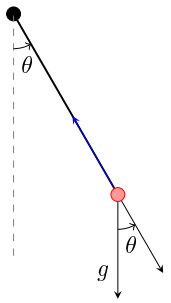
\includegraphics[height = 6cm]{figure1.png}
			\caption{A pendulum consisting of a weightless rod of length $L$ and a bob
				with a mass of $m$. The bob and the point of support are marked as a red
				and black dot, respectively. The parameter "g" denotes the gravational
				force. The angle $\theta$ is measured in the counterclockwise direction. Stable
				and unstable equilibrium points appear at $\theta = 0$ and $\theta = \pi$, respectively}
		\end{figure}
		\newpage
		\begin{enumerate}[label = (\alph*)]
			\item Perform a linear stability analysis in each of Eqs. (1.3)-(1.5).
			\begin{itemize}
				\item[(1.3) ] We can find the eigenvalues from solving its characteristic equation.
				\[\lambda^2 - 1 = 0\]
				Thus our eigenvalues are $\lambda = \pm 1$. This means that we get a \textbf{Saddle Point}.
				\item[(1.4) ] We can find the eigenvalues from solving its characteristic equation.
				\[\lambda^2 + \epsilon \lambda  - 1 = 0\]
				Thus our eigenvalues are $\frac{1}{2}\left(-\epsilon \pm \sqrt{\epsilon^2 + 4}\right)$.
				\\ \\
				Because $\sqrt{\epsilon^2 + 4} > |\epsilon| \geq 0$ for all values of $\epsilon$, we will always get a $\lambda_1 > 0$ and a $\lambda_2 < 0$, thus giving us a \textbf{Saddle Point}
				\\ \\
				\item[(1.5) ] Let $\zeta = z'$ and $\zeta' = z\left(1 -\frac{z^2}{6}\right)$.
				\[X' = \begin{pmatrix}
					\zeta \\ \zeta'
				\end{pmatrix} = \begin{pmatrix}
					0 & 1 \\
					1 -\frac{z^2}{6} & 0
				\end{pmatrix}\begin{pmatrix}
					z \\ \zeta
				\end{pmatrix}\]
				Notice we can find the critical points:
				\[X' = \begin{pmatrix}
					0 \\ 0
				\end{pmatrix} = \begin{pmatrix}
					0 & 1 \\
					1 -\frac{z^2}{6} & 0
				\end{pmatrix}\begin{pmatrix}
					z \\ \zeta
				\end{pmatrix}\]
				From this we get the following critical points: $(z,\zeta) = (\pm \sqrt{6},0)$ and $(z,\zeta) = (0,0)$.
				\\ \\
				Now notice the Jacobian:
				\[J(z, \zeta) = \left[\begin{array}{cc}
					\frac{d\zeta}{dz} & \frac{d\zeta}{dz'} \\
					\spacer \frac{d\zeta'}{dz} & \frac{d\zeta'}{dz'}	
				\end{array}\right] = \left[\begin{array}{cc}
					0 & 1 \\
					\spacer 1 - \frac{z^2}{2} & 0
				\end{array}\right]\]
				Notice the Jacobians and eigenvalues evaluated at the critical points:
				\[J(0,0) = \begin{bmatrix}
					0 & 1 \\ 1 & 0
				\end{bmatrix}\]
				From solving $|J - \lambda I| = 0$, we get that $\lambda = \pm 1$.  Thus we get a \textbf{Saddle Point}
				\[J(\pm \sqrt{6},0) = \begin{bmatrix}
					0 & 1 \\ -2 & 0
				\end{bmatrix}\]
				From solving $|J - \lambda I| = 0$, we get that $\lambda = \pm 2i$.  Thus we get a \textbf{Clockwise Center}
			\end{itemize}
			\newpage
			\item Compute potential energy functions for Eqs. (1.3) and (1.5). Find extrema of the potential energy functions to reveal the stability of equilibrium points.
			\\ \\
			Notice that in the following equation:
			\[\frac{d^z}{dt^2} + h(x\left(\frac{dz}{dt}\right) + g(z)\]
			we get the following:
			\[G(z) = \int g(z)\,dz \text{ represents potential energy}\]
			\[E\left(z, \frac{dz}{dt}\right) = \frac{1}{2}\left(\frac{dz}{dt}\right)^2 + G(z) \text{ represents total energy}\]
			\\ 
			So notice the potential energy function for Eq (1.3):
			\[G(z) = \int g(z)\,dz = \int -z \, dz = \frac{-z^2}{2}\]
			Notice that $G(z)$ has a equilibrium point at $z = 0$.  Noticing the PE function $G(z)$, we can see that at $z = 0$, there lies a local maxima, thus concluding that $z = 0$ is an \textbf{Unstable Equilibrium Point}
			\\ \\
			Notice the potential energy function for Eq (1.5):
			\[G(z) = \int g(z)\,dz = \int \left( -z + \frac{z^3}{6}\right) \, dz = \frac{-z^2}{2} + \frac{z^4}{24} = \frac{-z^2}{2}\left(1 - \frac{z^2}{12}\right)\]
			Notice that $G(z)$ has a equilibrium point at $z = 0$ and $z = \pm \sqrt{6}$.  We can see that at $z = 0$, $G(z)$ has a local maxima, indicating to us that $z = 0$ is an \textbf{Unstable Equilibrium Point}.  We can see at $z = \pm \sqrt{6}$, $G(z)$ has a local minima, indicating to us that $z = \pm \sqrt{6}$ is a \textbf{Stable Equilibrium Point} 
			\newpage
			\item Discuss the concept of structural stability using results in (1a)
			and (1b).
			\\ \\
			Structural Stability is when the linear stability can withstand small changes in perturbation without changing. A linear flow is structurally stable if and only if it is hyperbolic, meaning not having real parts zero. 
	 		\\ \\
	 		For equation (1.3), the stability was a saddle point at $z = 0$, so it is \textbf{Structurally Stable}. However, we got at $z = 0$ was an \textbf{Unstable} critical point for the potential energy function. 
	 		\\ \\
	 		For equation (1.5), the stability was a saddle point at the origin so it is \textbf{Structurally Stable} at that point.  At $z = \pm \sqrt{6}$, we got the stability was center, so it is \textbf{Structurally Unstable} at this point. However, we got at $z = 0$ was an \textbf{Unstable} critical point for the potential energy function, and at $z = \pm \sqrt{6}$ was a \textbf{Stable} critical point for the potential energy function.
	 		\\ \\
	 		This has to do with Structural stability being the linear stability, or in this case the derivative of potential energy, withstanding small changes in perturbation without changing.  Whereas, a stability of the equilibrium points of the potential energy function has to do with the function in itself  withstanding small changes in perturbation without changing. Notice how the changes in the derivative of potential energy at the critical points.  For equation (1.3) and (1.5), at $z = 0$, the concavity doesn't change thus indicating no sign change in the derivative of potential energy which would imply structural stability, despite $z = 0$ being an unstable maxima. For equation (1.5), at $z = \pm \sqrt{6}$, the concavity does change thus indicating a sign change in the derivative of potential energy which would imply structural instability, despite $z = \pm \sqrt{6}$ being a stable maxima.
	 		\begin{figure}[h!]
	 			\centering
	 			\begin{subfigure}{.45\textwidth}
	 				\centering
	 				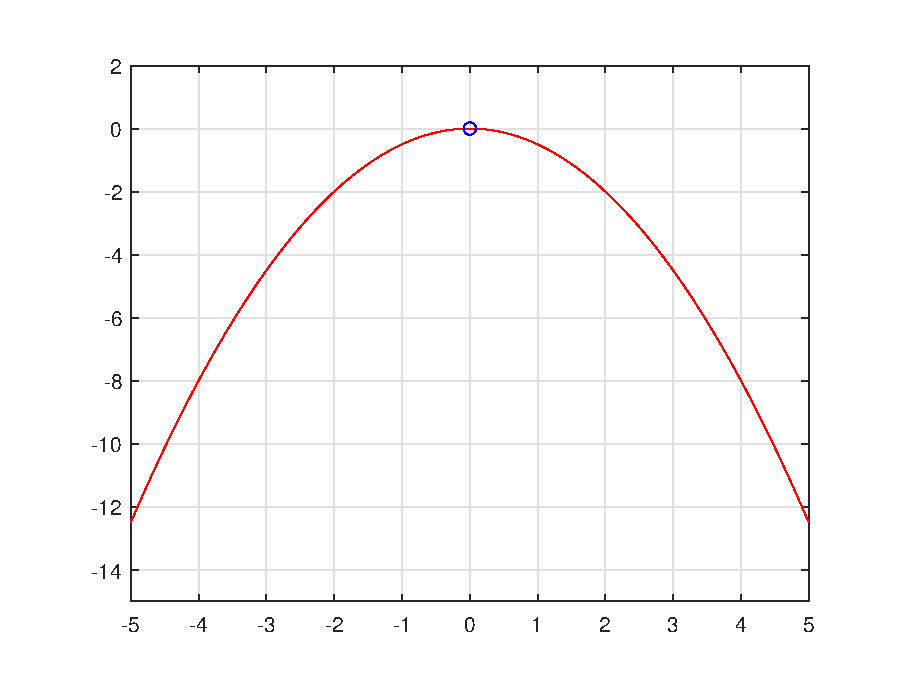
\includegraphics[height = 6cm]{Plots/eq13}
	 				\caption{PE 1.3}
	 			\end{subfigure}
	 			\begin{subfigure}{.45\textwidth}
	 				\centering
	 				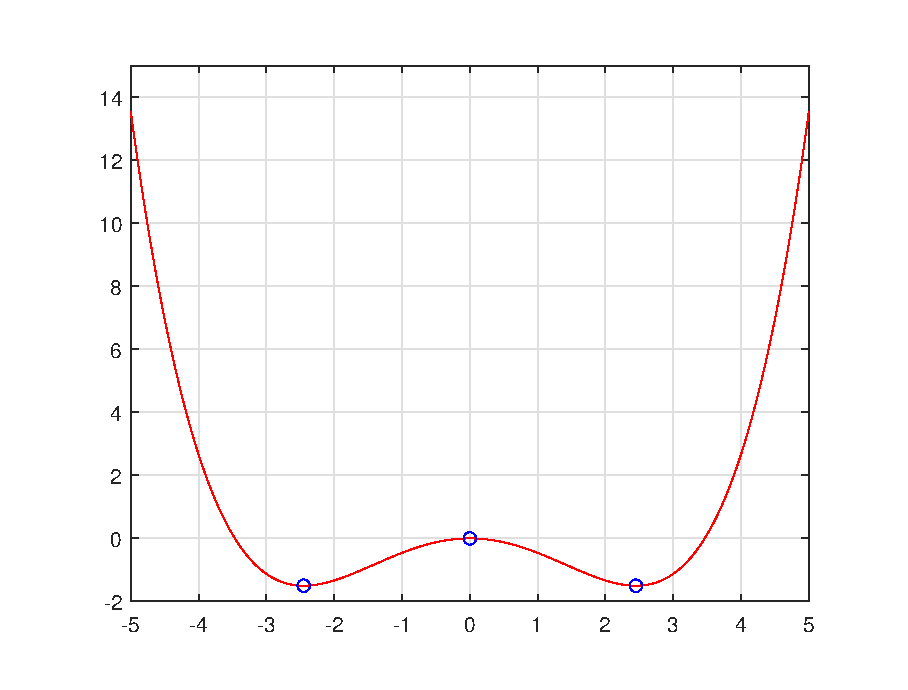
\includegraphics[height = 6cm]{Plots/eq15}
	 				\caption{PE 1.5}
	 			\end{subfigure}
	 		\end{figure}
		\end{enumerate}
	\end{problem}

	\begin{problem}{2}
		Complete a "mini report" based on the one slide summary (as
		shown in Figure 2). The following instructions are recommended.
		\begin{enumerate}[label = (\alph*)]
			\item Finish a one-paragraph summary.
			\\ \\
			The one slide summary shows all the various types of ODE's that we have covered within the semester. This includes two types of first order ODE's, a logistic equation and a limit cycle equation.  The summary also covers the second order ODE's, which is converted into a system of two first order ODE's.  The column following shows the solution of getting eigenvalues from a system of first order ODE's.  The summary covers non linear ODE's and gives two types, the DE-sech and DE-sec$\text{h}^2$. The following columns covers the steps towards the solution of the nonlinear ODE's, which would be to convert into a system of first order ODE's and then compute the Jacobian to find stability and eigenvalues. 
			\\
			\item Briefly summarize the major features of the 1st order ODEs
			(i.e., the column A), including stability of critical points, characteristics
			of solutions, the relation between the first and second ODEs, etc.
			\\ \\
			First order ODE's can be described as equations that's highest derivative order being one.  There are many ways to solve these types of ODE's.  For example, you can use the method of separability, method of exact equations, or the Bernoulli's method.  We find critical points by solving when the first derivative of dependent variable is equal to 0 (i.e. $y' = 0$).  The critical points have 3 types of stability, which are stable, unstable, and half stable.  We determine stability of first order ODE's by seeing when the first derivative of the dependent variable is greater than or less than 0 (ie $y' < 0$ or $y' > 0$).  Stable solutions show that over the independent variable, the solution tends towards the critical point, at which we call a stable node or sink.  Whereas, unstable solutions show that the solution tends away from the critical point, which we call an unstable node or source. Half stable solutions tend to go towards the critical point on one side of the critical point, and away on the other side, which we call a saddle point.
			\\ \\
			We can take a look at the two equations given in the summary and examine their solutions.  When we solve for the solution of logistic equations, we get something called a sigmoid function, a function in which as $t \mapsto \infty$, $y \mapsto 1$, and as $t \mapsto -\infty$, $y \mapsto 0$.  When we solve for the solution of the other first order ODE with degree 3, we get a limit cycle solution, or an isolated closed path.  A unique thing that happens for limit cycles is that we get a sink and a source towards the critical point.  Where the two solutions converge is the limit cycle, or closed path. 
			\newpage
			\item Discuss how to analyze a system of linear ODEs (i.e., expanding the information in the columns B and C).
			\\ \\
			When given a second order differential equation, we can expand it into a system of first order differential equations.  That is we introduce a new dependent variable, $y$, that we let equal to the derivative of the original dependent variable, $x$.  From here, the second derivative of the original dependent variable becomes simply the first derivative of the new dependent variable.  From here, we can isolate the first derivative of the new dependent variable in terms of the original variable and the new variable.  This gives us two first order differential equations as seen in the bottom portion of column B. We can find the critical points by solving the system when $X' = 0$, that is when each equation of the system equals 0. From here, we simply find the eigenvalues of this system by letting the $AX = \lambda X$, where A is the system's coefficient matrix and $\lambda$ is a diagonal matrix holding the systems eigenvalues.  We can solve that equality by taking solving $|A-\lambda I| = 0$.  This equality is known as the characteristic equation. Depending on the type of eigenvalues \{real and non repeating, real and repeating, and complex conjugates\}, we get three different type of solutions. 
			\[\lambda_1 \not = \lambda_2, \qquad \lambda_1, \lambda_2 \in \mathbb{R}, \qquad x = c_1e^{\lambda_1 t} + c_2e^{\lambda_2 t}  \]
			\[\lambda_1 = \lambda_2, \qquad \lambda_1, \lambda_2 \in \mathbb{R}, \qquad x = c_1e^{\lambda_1 t} + c_2te^{\lambda_2 t} + c_2e^{\lambda_2 t}  \]
			\[\lambda_1 = \bar{\lambda_2}, \qquad \lambda_1, \lambda_2 \in C, \qquad x = c_1e^{Re(\lambda_1)}\cos(Im(\lambda_1\,t)) + ic_2e^{Re(\lambda_1)}\sin(Im(\lambda_1\,t))\]
			We can also determine the stability based on these eigenvalues. If the eigenvalues are real and different, then there are a few stabilities for it.  If $\lambda_1 < 0$ and $\lambda_2 < 0$, then we get a stable sink around the critical point. If $\lambda_1 > 0$ and $\lambda_2 > 0$, then we get an unstable source around the critical point. If $\lambda_1 < 0$ and $\lambda_2 > 0$, then we get a saddle point around the critical point. 
			\newpage
			\item Briefly summarize the major features of the 2nd order nonlinear ODEs (i.e., the column D), including stability of critical points, the relation among them, etc.
			\\ \\
			When it comes to 2nd order nonlinear ODE's, we can still split the ODE into 2 first order ODE's.  We do however, get the dependent variable in the matrix, so we need to find the critical points of 2D system. Once we've found the critical points, we can evaluate the Jacobian at those points, to give us a matrix in which we can solve for eigenvalues with.  From there, we can see the stability at those critical points.  By introducing new variables into first order logistic equations, we can convert them into a DE-sec$\text{h}^2$, which is a differential equation with solutions as a hyperbolic secant square function, such as the Korteweg-de Vries (KdV) equation in a traveling-wave coordinate
			\item Discuss how to analyze a system of nonlinear high-order ODEs (e.g., stability analysis, a energy method, a perturbation method, the WKBJ or LG method, etc.)
	 		\\ \\
	 		When given a system of nonlinear high-order ODE's, we can use various methods to approximate the solution.  To analyze the stability, we can find the eigenvalues of a multi dimensional system, and use the same stability analysis said in parts above. We can use perturbation theory to solve these ODE's.  That it we choose a very small perturbation variable $\epsilon$, we can see small changes in the dependent variable as we make small changes in the independent variable. We can use the WKBJ method, where we let the dependent variable, $y$ be an exponential function, $e^{S(x)}$.  From here, we can plug this into the ODE and solve for $S(x)$.  We solve for $S(x)$ by using the method of Dominant Balance, which allows us to zero out very small terms as $x \mapsto \infty$.
		\end{enumerate}
		\begin{figure}[b!]
			\centering
			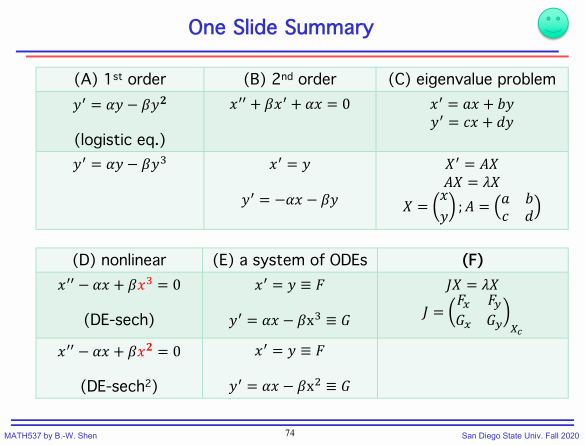
\includegraphics[height = 10cm]{figure2.png}
			\caption{One slide summary ($\alpha > 0$ and $\beta > 0$)}
		\end{figure}
	\end{problem}

	\begin{problem}{4}
		Consider a boundary-layer problem with the following second order linear differential equation:
		\[\epsilon\frac{d^2y}{dx^2} +  (1 + \epsilon)\frac{dy}{dx} + y = 0, \qquad y(0) = 0, \wspace y(1) = 1.\]
		\\ \\
		Apply the boundary layer method to solve the above equation for
		\begin{enumerate}[label = (\alph*)]
			\item the inner solution in the inner region;
			\item the outer solution in the outer region;
			\item the solution ($y_{match}$) in the overlap region;
			\item the uniform approximation ($y_{unif}$) to $y$ (i.e., $y_{unif} ~ y$). \\
		\end{enumerate}
		\newpage
		Notice the following
		\[y_{out} ~ \sum_{n=0}^{\infty} y_n \epsilon^n = y_0 + \epsilon y_1 + \epsilon^2 y_2 + \cdots + e^{n}y_n\]
		Using the boundary condition that $y(1) = 1$, we get that
		\[y_0(1) = 1, \qquad y_1(1) = 0, \qquad y_2(1) = 0, \quad \cdots \quad y_n(1) = 0\]
		From here if we resubstitute $y_{out}$ into our original equation, we get:
		\begin{align*}
			\epsilon\bigg(y_0'' &+ \epsilon y_1'' + \epsilon^2 y_2'' + \cdots + e^{n}y_n''\bigg) + \epsilon\bigg(y_0' + \epsilon y_1' + \epsilon^2 y_2' + \cdots + e^{n}y_n'\bigg) \\
			&+\bigg(y_0' + \epsilon y_1' + \epsilon^2 y_2' + \cdots + e^{n}y_n'\bigg) + \bigg(y_0 + \epsilon y_1 + \epsilon^2 y_2 + \cdots + e^{n}y_n\bigg) = 0
		\end{align*}
		Notice we can rearrange this into:
		\begin{align*}
			\bigg(y_0' + y_0\bigg) &+ \bigg(\epsilon y_1' + \epsilon^2 y_2' + \cdots + e^{n}y_n'\bigg) + \bigg(\epsilon y_1 + \epsilon^2 y_2 + \cdots + e^{n}y_n\bigg) \\
			&= -\bigg(\epsilon y_0'' + \epsilon^2 y_1'' + \epsilon^3 y_2'' + \cdots + e^{n+1}y_n''\bigg) - \bigg(\epsilon y_0' + \epsilon^2 y_1' + \epsilon^3 y_2' + \cdots + e^{n+1}y_n'\bigg)
		\end{align*}
		Now if we compare each corresponding term in relation to its order, we get the following:
		\begin{align*}
			O(\epsilon^0) \qquad y_0' + y_0 &= 0 \\
			O(\epsilon) \qquad y_1' + y_1 &= -y_0'' - y_0' \\
			O(\epsilon^n) \qquad y_n' + y_n &= -y_{n-1}'' - y_{n-1}'
		\end{align*}
		If we solve $y_0' + y_0 = 0$, we get $y_0 = Ce^{-x}$. Using the initial condition, we get:
		\[y_0 = e^{1-x}\]
		From this, we get the following:
		\begin{align*}
			y_1' + y_1 &= -y_0'' - y_0' \\
			&= -\frac{d}{dx}\bigg(y_0' + y_0\bigg) = 0
		\end{align*}
		So we get $y_1' + y_1 = 0$, which solves to be $y_1 = Ce^{-x}$. Using the initial condition, we get:
		\[y_1 = 0e^{-x} = 0\]
		\textbf{Now if we do keep doing this recursively, we get the following solution:}
		\begin{align*}
			\boldsymbol{y_{out} ~ \sum_{n=0}^{\infty} y_n \epsilon^n} &= \boldsymbol{y_0 + \epsilon y_1 + \epsilon^2 y_2 + \cdots + e^{n}y_n} \\
			&= \boldsymbol{e^{1-x} + 0 + \cdots + 0} \\
			&= \boldsymbol{e^{1-x}}
		\end{align*}
		\newpage
			We first need to apply some "rescaling", so we let:
		\[x = \epsilon\X \qquad \frac{d}{dx} = \frac{1}{\epsilon}\frac{d}{d\X} \qquad \frac{d^2}{dx^2} = \frac{1}{\epsilon^2}\frac{d^2}{d\X^2}\]
		We also let $\Y(\X) = y(x)$.  This will give us the following:
		\[\epsilon \frac{1}{\epsilon^2}\frac{d^2\Y}{d\X^2} + \frac{1}{\epsilon}\frac{d\Y}{d\X} + \epsilon\frac{1}{\epsilon}\frac{d\Y}{d\X} + \Y = \frac{1}{\epsilon}\left(\frac{d^2\Y}{d\X^2} + \frac{d\Y}{d\X}\right) + \frac{d\Y}{d\X} + \Y = 0 \]
		Now we get the following:
		\[\Y ~ \sum_{n=0}^{\infty} \Y_n \epsilon^n = \Y_0 + \epsilon \Y_1 + \epsilon^2 \Y_2 + \cdots + e^{n}\Y_n\]
		Now if we substitute this into our equation, we get:
		\begin{align*}
			\bigg(\epsilon^{-1}\Y_0'' + \epsilon^{-1}\Y_0'\bigg) &+ \bigg(\Y_1'' + \epsilon\Y_2'' + \cdots + \epsilon^{n-1}\Y_n''\bigg) + \bigg(\Y_1' + \epsilon\Y_2' + \cdots + \epsilon^{n-1}\Y_n'\bigg) \\
			&= -\bigg(\Y_0' + \epsilon \Y_1' + \epsilon^2 \Y_2' + \cdots + e^{n}\Y_n'\bigg) - \bigg(\Y_0 + \epsilon \Y_1 + \epsilon^2 \Y_2 + \cdots + e^{n}\Y_n\bigg)
		\end{align*}
		Now if we compare each corresponding term in relation to its order, we get the following:
		\begin{align*}
			O(\epsilon^{-1}) \qquad \Y_0'' + \Y_0' &= 0 \\
			O(1) \qquad \Y_1'' + \Y_1' &= -\Y_0' - \Y_0 \\
			O(\epsilon^{n}) \qquad \Y_{n+1}'' + \Y_{n+1}' &= -\Y_{n}' - \Y_{n}
		\end{align*}
		Notice the following solution:
		\begin{align*}
			\Y_0'' + \Y_0' &= 0 & \ln \Y_0' &= -\X + c_1 \\
			\Y_0'' &= -\Y_0' &  \int \Y_0' &= \int c_2e^{-\X}  \\
			\int \frac{\Y_0''}{\Y_0'} &= -\int \,d\X & \Y_0 &= c_1 + c_2e^{-\X}
		\end{align*}
		Using the initial conditions, we get that $c_1 = -c_2$, such that:
		\[\Y_0 = A_0\bigg(1 - e^{-\X}\bigg)\]
		Now we solve the following:
		\[\Y_1'' + \Y_1' = -\Y_0' - \Y_0\]
		First we find the homogeneous solution:
		\begin{align*}
			\Y_{1h}'' + \Y_{1h}' &= 0 & \ln \Y_{1h}' &= -\X + d_1 \\
			\Y_{1h}'' &= -\Y_{1h}' &  \int \Y_{1h}' &= \int d_2e^{-\X}  \\
			\int \frac{\Y_{1h}''}{\Y_{1h}'} &= -\int \,d\X & \Y_{1h} &= d_1 + d_2e^{-\X}
		\end{align*}
		Using the initial conditions, we get that $d_1 = -d_2$, such that:
		\[\Y_{1h} = A_1\bigg(1 - e^{-\X}\bigg)\]
		Next we solve for the particular solution:
		\begin{align*}
			\Y_1'' + \Y_1' &= -\Y_0' - \Y_0 \\
			&= -\bigg(A_0e^{-\X}\bigg) - \bigg(A_0 - A_0e^{-\X}\bigg) \\
			&= -A_0
		\end{align*}
		Now we let $\Y_{1p} = C\X$, such that $\Y_{1p}' = C$, and $\Y_{1p}'' = 0$.
		\[\Y_{1p}'' + \Y_{1p}' = -A_0, \qquad C = -A_0\]
		Thus we get the particular solution:
		\[\Y_{1p} = -A_0\X\]
		Finally, we get the following:
		\[\Y_{1} = \Y_{1h} + \Y_{1p} = A_1\bigg(1 - e^{-\X}\bigg) - A_0\X\]
		Thus we get the following solution for $\Y$:
		\[\Y ~ A_0\bigg(1 - e^{-\X}\bigg) + \epsilon\bigg(A_1\bigg(1 - e^{-\X}\bigg) - A_0\X\bigg) + \cdots\]
		\newpage
		Notice the following solutions:
		\begin{align*}
			\Y &~ A_0\bigg(1 - e^{-\X}\bigg) + \epsilon\bigg(A_1\bigg(1 - e^{-\X}\bigg) - A_0\X\bigg) + \cdots \\
			y_{out} &~ e^{1-x}
		\end{align*}
		Notice we can rewrite the outer solution:
		\[y_{out} ~ e^{1-x} = ee^{-x} = ee^{-\epsilon\X} = e\bigg(1 - \epsilon\X + \frac{(\epsilon\X)^2}{2} + \cdots \bigg) = e - e\epsilon\X + e\frac{(\epsilon\X)^2}{2} + \cdots + (-1^n)e\frac{\epsilon^n \X^n}{n!}\]
		From here, we can match the inner and outer solutions such that:
		\begin{align*}
			\Y_0 = A_0\bigg(1 - e^{-\X}\bigg) &= e \qquad \X \rightarrow \infty \qquad A_0 = e \\
			\Y_1 = A_1\bigg(1 - e^{-\X}\bigg) - A_0\X &= -e\X \qquad \X \rightarrow \infty \qquad A_1 = 0
		\end{align*}
		Notice the following statements after matching:
		\begin{align*}
			\Y_0 &= e\bigg(1 - e^{-\X}\bigg) = e - e^{1 - \X} \\
			\Y_1 &= -e\X \\
			\Y_n &= e\frac{-1^n\X^n}{n!}
		\end{align*}	
		\textbf{Resubstituting this we get the inner solution:}
		\begin{align*}
			\boldsymbol{y_{in} = \Y} &~ \boldsymbol{e - e^{1 - \X} - \epsilon e\X + \cdots +  (-1^n)e\frac{\epsilon^n \X^n}{n!}} \\
			&~ \boldsymbol{- e^{1 - \X} + \left(e - \epsilon e\X + \cdots +  (-1^n)e\frac{\epsilon^n \X^n}{n!}\right)} \\
			&~ \boldsymbol{-e^{1-\X} + e^{1 - \epsilon \X}} \\
			&~ \boldsymbol{-e^{1-\X} + e^{1 - x}}
		\end{align*}
		\textbf{\boldmath Notice the solution in the overlap region can be found by seeing how $y_{out}$ and $y_{in}$ "match".  Thus we get:}
		\[\boldsymbol{y_{match} = e^{1-x}}\]
		\textbf{Lastly, the uniform approximation is just the sum of the inner and outer solutions minus the overlap region:}
		\[\boldsymbol{y_{unif} = y_{in} + y_{out} - y_{match} = y_{in} = -e^{1-\X} + e^{1 - x}}\]
	
	\end{problem}


\end{document}
